\documentclass[12pt]{article}
\usepackage{amsmath}
\usepackage{amssymb}
\usepackage{fullpage}
\usepackage{setspace}
\usepackage{graphicx}
\usepackage{natbib}
\usepackage{color}
\usepackage{listings}
\usepackage{float}
\usepackage{subfig}
\usepackage{caption}
\usepackage{multirow}
\usepackage{rotating}
\usepackage{tikz}
\usepackage{soul}
\usepackage{ulem}

% \newcommand\hi[1]{\colorbox{yellow}{\textcolor{black}{#1}}}

\newcommand{\todo}[1]{\textcolor{red}{#1}}
\definecolor{mylightblue}{RGB}{123,146,210} % This is an example RGB for light blue

\begin{document}

% set the h1 highlight color to light green-blue (set a custom rgb color)
\definecolor{orange}{RGB}{255,186,150}
\sethlcolor{orange}

\usetikzlibrary{calc, patterns, patterns.meta}

\title{CVT: Thoughts and a Proposed Design}
\author{Nikhil Vijay}
\date{\today}
\maketitle

\begin{abstract}
  This document is a collection of my initial thoughts and ideas on CVT systems, their uses, what we want from them, and my idea for one. My idea is a dual-differential CVT system, which is a single-input and single-output CVT system that uses two differentials: one to split the input power into a high and low speed reducers (creating a power differential) and one to combine them again. It may have been done before (and I have found evidence for this), but I believe those explorations lack depth.
\end{abstract}

\section{Why are CVTs Useful?}
\subsection{Mechanical Power}
The mechanical power of some rotating thing is given by the following equation:
\begin{equation}
  P_{m} = \tau\cdot\omega
\end{equation}

You can think of $\tau$ (torque) and $\omega$ (speed) as the length and width of a rectangle, the rectangle would have an area of $P_{m}$. 

% Figure 1: Rectangular representation of mechanical power.
\begin{figure}[H]
  \centering
  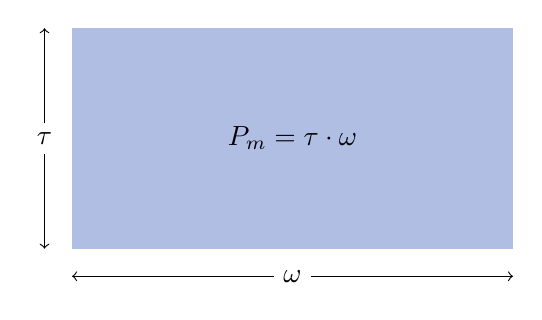
\begin{tikzpicture}[scale=0.7]
    % Define length and width
    \def\width{4}
    \def\length{2*\width} % width is twice the length to maintain 1:2 aspect ratio

    % Draw blue rectangle with aspect ratio of 1:2
    \fill[mylightblue, fill opacity=0.6] (0,0) rectangle (\length,\width);

    % Draw measurement line for tau with central label
    \draw [<->] (-0.5,0) -- (-0.5,\width) node [midway, fill=white] {$\tau$};

    % Draw measurement line for omega with central label
    \draw [<->] (0,-0.5) -- (\length,-0.5) node [midway, fill=white] {$\omega$};
    
    % Add text inside the rectangle
    \node at (\length/2,\width/2) {$P_m = \tau \cdot \omega$};
  \end{tikzpicture}
  \caption{Rectangular representation of mechanical power.}\label{fig:power_rectangle}
\end{figure}

If we fixed $P_{m}$ to be some constant, there would be an infinite number of rectangles with that area, and thus there are an infinite number of $\tau:\omega$ ratios for any $P_{m}$. Each of these rectangles is representative of one single gear ratio. 

% Figure 2: Various examples of rectangles with the same area Pm.
\begin{figure}[H]
  \centering
  \resizebox{0.75\textwidth}{!}{%
  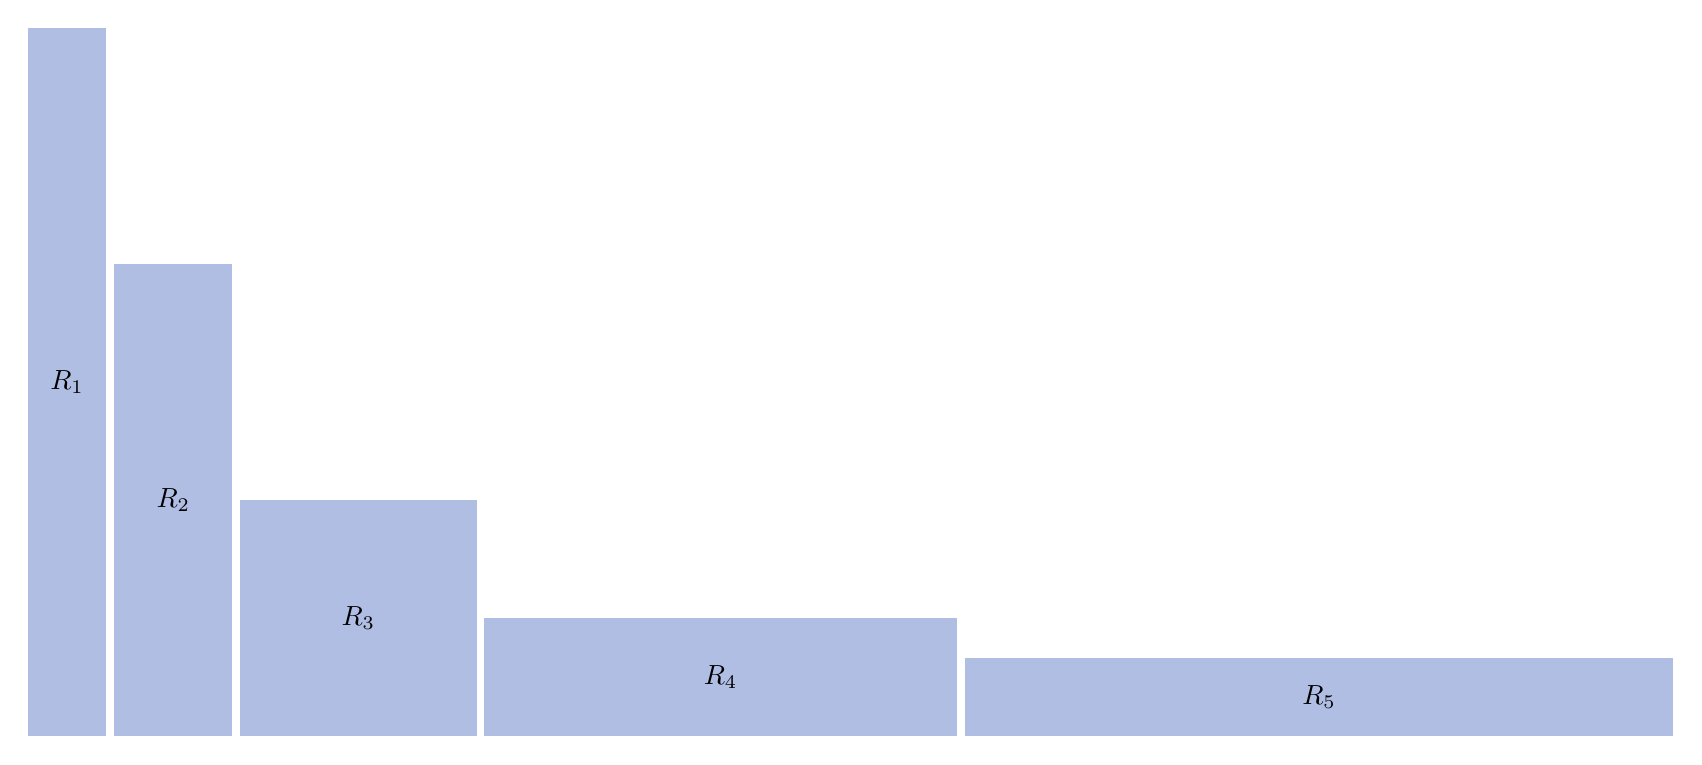
\begin{tikzpicture}
    % Define the consistent area for the rectangles
    \pgfmathsetmacro{\area}{9} % The area of each rectangle
    
    % Calculate widths and heights based on the given ratios
    \pgfmathsetmacro{\widthOne}{sqrt(\area / 9)}
    \pgfmathsetmacro{\heightOne}{\widthOne * 9}
    
    \pgfmathsetmacro{\widthTwo}{sqrt(\area / 4)}
    \pgfmathsetmacro{\heightTwo}{\widthTwo * 4}
    
    \pgfmathsetmacro{\widthThree}{sqrt(\area)} % This will be a square
    \pgfmathsetmacro{\heightThree}{\widthThree}
    
    \pgfmathsetmacro{\widthFour}{sqrt(\area * 4)}
    \pgfmathsetmacro{\heightFour}{\area / \widthFour}
    
    \pgfmathsetmacro{\widthFive}{sqrt(\area * 9)}
    \pgfmathsetmacro{\heightFive}{\area / \widthFive}
    
    % Horizontal gap between rectangles
    \newcommand{\gap}{0.1}
    
    % Draw all rectangles with labels centered
    \newcommand{\drawRectangle}[4]{% width, height, position, label
      \pgfmathsetmacro{\posX}{\lastX + \lastWidth + \gap} % Set X position
      \fill[mylightblue, fill opacity=0.6] (\posX,0) rectangle ++(#1,#2);
      \node at (\posX + #1/2,#2/2) {#3};
      \global\let\lastWidth=#1 % Update last width
      \global\let\lastX=\posX % Update last X position
    }
    
    % Initialize last width and X position
    \newcommand{\lastWidth}{0}
    \newcommand{\lastX}{-\gap} % Start with negative gap to compensate for initial addition
    
    % Draw rectangles
    \drawRectangle{\widthOne}{\heightOne}{\(R_1\)};
    \drawRectangle{\widthTwo}{\heightTwo}{\(R_2\)};
    \drawRectangle{\widthThree}{\heightThree}{\(R_3\)};
    \drawRectangle{\widthFour}{\heightFour}{\(R_4\)};
    \drawRectangle{\widthFive}{\heightFive}{\(R_5\)};
    
    % Total width of all rectangles and gaps
    \pgfmathsetmacro{\totalWidth}{\widthOne + \widthTwo + \widthThree + \widthFour + \widthFive + 4*\gap}
  \end{tikzpicture}
  } % end of \resizebox
  \caption{Various examples of rectangles with the same area $P_{m}$.}\label{fig:side_rects}
\end{figure}

Layering these rectangles gives us a crude approximation of a curve, where each $\omega$ (x-axis) has a corresponding $\tau$ (y-axis):

% Figure 3: Crude approximation of optimal power graph with 5 rectangles.
\begin{figure}[H]
  \centering
  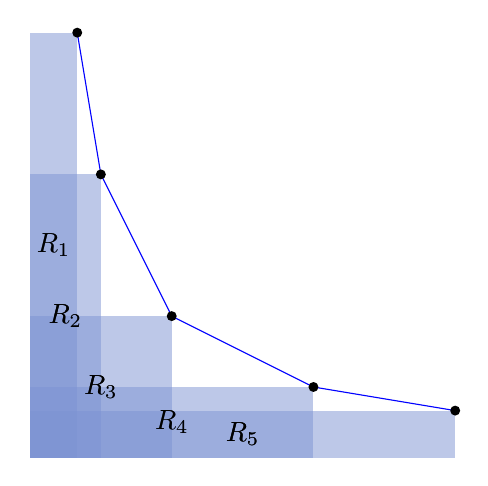
\begin{tikzpicture}[scale=0.6] % The scale can be adjusted for sizing
    % Define the consistent area for the rectangles
    \pgfmathsetmacro{\area}{9} % The area of each rectangle
    
    % Calculate widths and heights based on the given ratios
    \pgfmathsetmacro{\widthOne}{sqrt(\area / 9)}
    \pgfmathsetmacro{\heightOne}{\widthOne * 9}
    
    \pgfmathsetmacro{\widthTwo}{sqrt(\area / 4)}
    \pgfmathsetmacro{\heightTwo}{\widthTwo * 4}
    
    \pgfmathsetmacro{\widthThree}{sqrt(\area)} % This will be a square
    \pgfmathsetmacro{\heightThree}{\widthThree}
    
    \pgfmathsetmacro{\widthFour}{sqrt(\area * 4)}
    \pgfmathsetmacro{\heightFour}{\area / \widthFour}
    
    \pgfmathsetmacro{\widthFive}{sqrt(\area * 9)}
    \pgfmathsetmacro{\heightFive}{\area / \widthFive}
    
    % Draw the rectangles with transparency
    \fill[fill=mylightblue, fill opacity=0.5] (0,0) rectangle (\widthOne,\heightOne) node[pos=.5, opacity=1] {\(R_1\)};
    \fill[fill=mylightblue, fill opacity=0.5] (0,0) rectangle (\widthTwo,\heightTwo) node[pos=.5, opacity=1] {\(R_2\)};
    \fill[fill=mylightblue, fill opacity=0.5] (0,0) rectangle (\widthThree,\heightThree) node[pos=.5, opacity=1] {\(R_3\)};
    \fill[fill=mylightblue, fill opacity=0.5] (0,0) rectangle (\widthFour,\heightFour) node[pos=.5, opacity=1] {\(R_4\)};
    \fill[fill=mylightblue, fill opacity=0.5] (0,0) rectangle (\widthFive,\heightFive) node[pos=.5, opacity=1] {\(R_5\)};
  
  % Labels for rectangles
  \node[overlay] at (\widthOne/2, \heightOne/2) {\(R_1\)};
  \node[overlay] at (\widthTwo/2, \heightTwo/2) {\(R_2\)};
  \node[overlay] at (\widthThree/2, \heightThree/2) {\(R_3\)};
  \node[overlay] at (\widthFour/2, \heightFour/2) {\(R_4\)};
  \node[overlay] at (\widthFive/2, \heightFive/2) {\(R_5\)};
  
  % Draw line segments connecting the top right corners of each rectangle
  \draw[thin, blue] (\widthOne,\heightOne) -- (\widthTwo,\heightTwo);
  \fill[black] (\widthOne,\heightOne) circle (3pt);
  \draw[thin, blue] (\widthTwo,\heightTwo) -- (\widthThree,\heightThree);
  \fill[black] (\widthTwo,\heightTwo) circle (3pt);
  \draw[thin, blue] (\widthThree,\heightThree) -- (\widthFour,\heightFour);
  \fill[black] ((\widthThree,\heightThree) circle (3pt);
  \draw[thin, blue] (\widthFour,\heightFour) -- (\widthFive,\heightFive);
  \fill[black] (\widthFour,\heightFour) circle (3pt);
  \fill[black] (\widthFive,\heightFive) circle (3pt);
  \end{tikzpicture}
  \caption{Crude approximation of optimal power graph with 5 rectangles.}\label{fig:layered_rects}
\end{figure}

Depending on the torque requirements, you could choose between discrete reduction ratios. This is how a conventional bicycle works with its chain and sprocket transmission and manual gear shifter.

\hl{If we had a bike transmission with an infinite amount of these sprockets, we wouldn't have to choose between a handfull of discrete, sub-optimal reduction ratios. Instead, we could just choose the exact ratio for our requirements. This is the idea for a CVT}.

Specifically extending the bicycle example, we would end up with something like the V-Belt CVTs we currently use in some cars. 

\subsection{Optimal Torque-Speed Curve w/ Fixed $P_{m}$}

We can bring this CVT idea back to the torque-speed graph by adding more and more rectangles (approaching infinity), giving us a continuous curve. This type of curve is aptly named: it is a rectangular hyperbola.

% Figure 4: Optimal torque-speed curve with a constant
\begin{figure}[H]
  \centering
  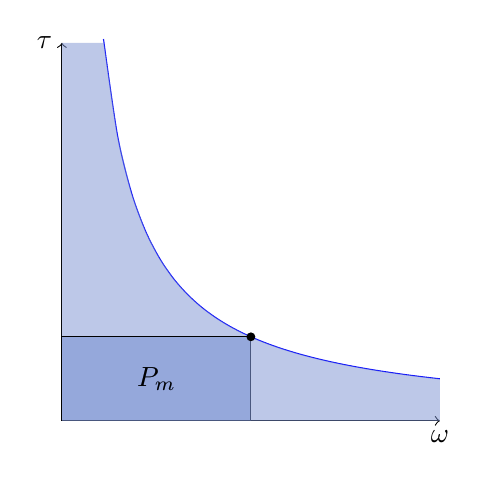
\begin{tikzpicture}[scale=1.6]
    % Define the area under the curve and the coordinates for the rectangle
    \pgfmathsetmacro{\a}{1.5}
    \pgfmathsetmacro{\b}{1/\a}
    \pgfmathsetmacro{\PmArea}{\a*\b} % The area of the rectangle under the curve
    
    % Draw the axes
    \draw[->] (0,0) -- (3,0) node[below] {$\omega$};
    \draw[->] (0,0) -- (0,3) node[left] {$\tau$};
    
    % Draw the curve
    \draw[domain=0.33:3,smooth,variable=\x,blue] plot ({\x},{1/\x});
    \fill[mylightblue, fill opacity=0.5] (0,0) -- (0,3) -- (0.33,3) -- plot[domain=0.33:3] (\x,{1/\x}) -- (3,0) -- cycle;
    
    % Draw the rectangle
    \draw[thin, black] (0,0) rectangle (\a,\b) node[pos=.5] {$P_m$};
    \fill[mylightblue, fill opacity=0.6] (0,0) rectangle (\a,\b) node[pos=.5] {$P_m$};

    
    
    % Draw the dot at the corner of the rectangle on the curve
    \fill[black] (\a,\b) circle (1pt);
    
    % Label the point
    \node[overlay] at (\a/2,\b/2) {$P_{m}$};
    \end{tikzpicture}
    \caption{Optimal torque-speed curve with a constant $P_{m}$}\label{fig:optimal_power_curve}
\end{figure}

This curve, the rectangular hyperbola (aka: $y=\frac{1}{x}$), is the ideal torque-speed curve in terms of power, we are always at peak performance. The function for this curve is 
\begin{equation}
  \tau = \frac{P_{m}}{\omega}
\end{equation}

Remember that $P_{m}$ is a constant.

\subsection{Torque-Speed Curve of a Motor}

\subsubsection{Basic Torque-Speed Graph}

One thing that can help our intution for this curve is looking at the torque-speed curve of a motor.

% Figure 5: Torque-speed curve of a motor from Adi Mehrotra’s Dynos for Dummies
\begin{figure}[H]
  \centering
  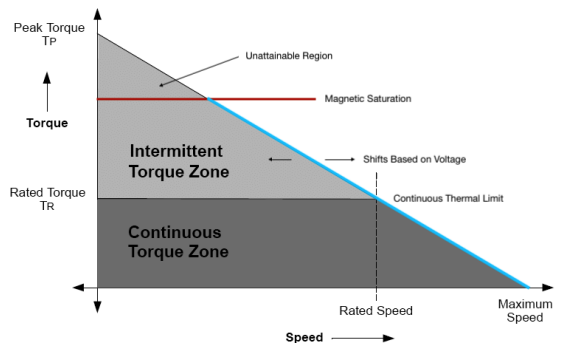
\includegraphics[width=0.75\textwidth]{motor-torque-speed.png}
  \caption{Torque-speed curve of a motor from Adi Mehrotra's Dynos for Dummies}\label{fig:dynos_for_dummies}
\end{figure}

This curve is a simple linear function, connecting the y-intercept (peak torque $\tau_{p}$ or $\tau_{\max}$) to the x-intercept (maximum speed $\omega_{\max}$). 

% Figure 6: Rectangular hyperbola and motor torque-speed curve.
\begin{figure}[H]
  \centering
  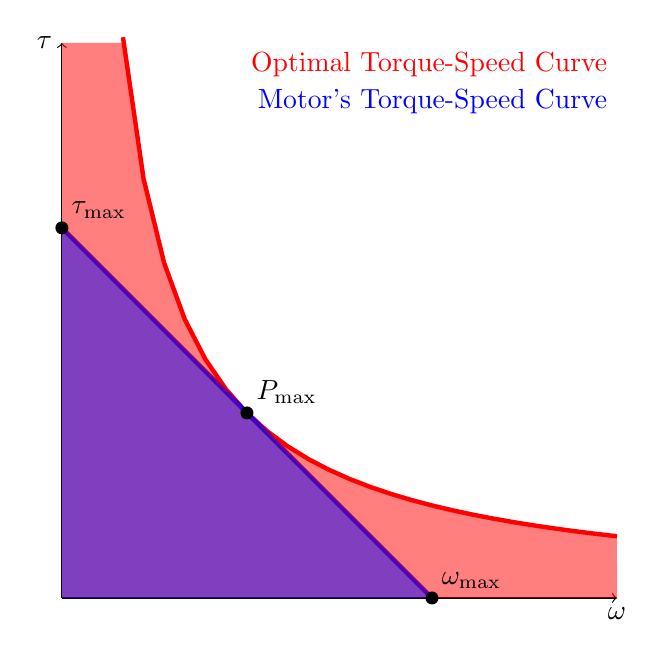
\begin{tikzpicture}[scale=2.35]
    % Define maximum values for torque (Tmax) and omega (ωmax)
    \pgfmathsetmacro{\Tmax}{2}
    \pgfmathsetmacro{\Omax}{2}
    
    % Define the point of maximum power Pmax
    \pgfmathsetmacro{\Pmax}{1} % Assumed for this example, adjust as needed
  
    % Draw the axes
    \draw[->] (0,0) -- (3,0) node[below] {$\omega$};
    \draw[->] (0,0) -- (0,3) node[left] {$\tau$};
    
    % Draw the optimal torque-speed curve (hyperbolic)
    \draw[domain=0.33:3,ultra thick,red] plot (\x,{1/\x});
  
    % Draw the motor's torque-speed curve (linear)
    \draw[domain=0:2,ultra thick,blue] plot (\x,{2-\x});
  
    \node[overlay, below left, red] at (3,3) {Optimal Torque-Speed Curve};
    \node[overlay, below left, blue] at (3,3-.2) {Motor's Torque-Speed Curve};
  
    
    % Shade the area under the motor's torque-speed curve
    \fill[red, fill opacity=0.5] (0,0) -- (0,3) -- (0.33,3) -- plot[domain=0.33:3] (\x,{1/\x}) -- (3,0) -- cycle;
  
    \fill[blue, fill opacity=0.5] (0,0) -- plot[domain=0:2] (\x,{2-\x}) -- (\Pmax,0) -- cycle;
    
    % Draw the dot at Pmax
    \fill[black] (1,1) circle (1pt) node[above right] {$P_{\max}$};
    
    % % Draw dashed lines to the axes
    % \draw[dashed] (1,0)  -- (1,1);
    % \draw[dashed] (0,1) -- (1,1);
  
    \fill[black] (2,0) circle (1pt) node[above right] {$\omega_{\max}$};
    \fill[black] (0,2) circle (1pt) node[above right] {$\tau_{\max}$};
  
  \end{tikzpicture}
  
  \caption{Rectangular hyperbola and motor torque-speed curve.}\label{fig:ts_comparisons}
\end{figure}

If you compare this to the rectangular hyperbola, we see that there is one point where they intersect, which is also the point of maximum power output for a motor.

\subsubsection{Motor Efficiency Graphs and CVT Use-Cases}
For the obvious use-case for CVT, where we want to use the maximum amount of power while the torque demands are varying (different terrains, driving uphill vs. downhill, etc.), we would always run our input at the speed at the intersection point, and then the transmission would vary the output speed depending on the exact torque demand.

However, what if we are driving on these different terrains, and there is a speed limit? Or a traffic light? In this case, we are not trying to maximize speed or power, we are trying to conserve energy, and almost never get to use $P_{\max}$ in the first place. It is an energy-efficiency optimization.

Energy efficiency, $\mu_{m}$, is defined as the ratio of mechanical power output to electrical power input. This means that we want to maximize $\mu_{m}$:
\begin{equation}
  \mu_{m} = \frac{P_{m}}{P_{e}}
\end{equation}

Usually, energy efficiency for a motor drops off significantly at lower speeds, while it increases at higher speeds. 

\begin{figure}[H]
  \centering
  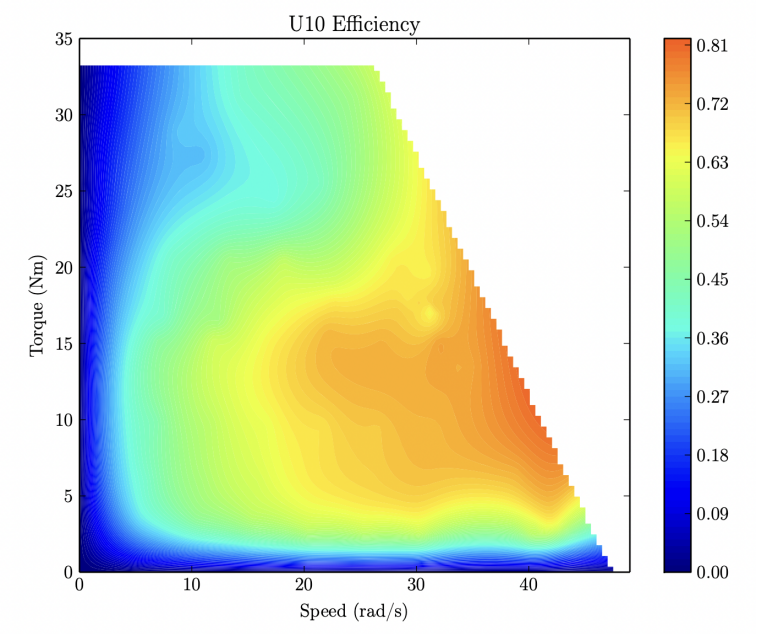
\includegraphics[width=0.75\textwidth]{motor-efficiency.png}
  \caption{The torque/speed/efficiency map for the U10 from Elijah Stanger-Jones’ masters thesis. (Found in Adi Mehrotra's Dynos for Dummies)}\label{fig:motor_efficiency}
\end{figure}

Thus, in the case of a vehicle forced to drive at low speeds, it would be beneficial to run the motor at a higher speed, and choose a reduction ratio that significantly decreases speed. Because we are already running our motor at a high speed, we have to be using $< P_{\max}$, and thus we would be using less energy.

There is an unfortunate issue related to this: it only goes one way. We can set our motor to run at a high speed, and choose to gear it down, maintaining high energy efficiency and low power at low speeds. But, if we set our motor at a low speed and geared it up, we could not expect high energy efficiency at high speeds, so we would benefit by simply running our motor at a higher speed and gearing closer to a 1:1 reduction. Thankfully, running our motor at those high speeds is already more efficient, so we are not losing much.

\section{CVT Design}

\subsection{Constraints}

Going back to the bike chain and sprocket example, I earlier explained that we could ``have an infinite number of sprockets'', and that would yield a CVT. That is actually not true. What I really meant was an infinite amount of sprockets \textbf{between} two discrete sizes, the largest and a smallest. 

We want the curve to be the continous on a closed interval $[\omega_{1},\omega_{2}]$, where $\omega_{1}$ is the minimum expected operating speed, and $\omega_{2}$ is the maximum expected operating speed. 

\begin{figure}[H]
  \centering
  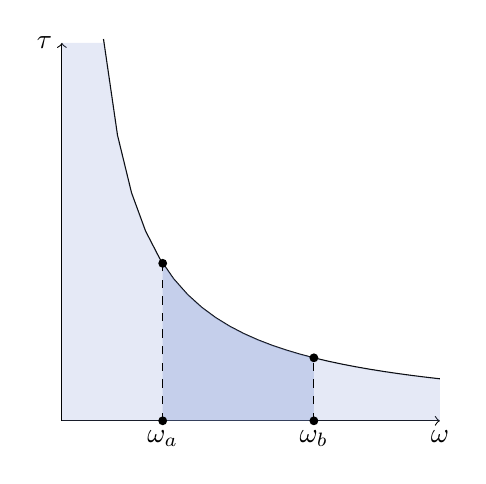
\begin{tikzpicture}[scale=1.6]
    % Define maximum values for torque (Tmax) and omega (ωmax)
    \pgfmathsetmacro{\Tmax}{2}
    \pgfmathsetmacro{\Omax}{2}
    
    % Define the point of maximum power Pmax
    \pgfmathsetmacro{\Pmax}{1} % Assumed for this example, adjust as needed
  
    % Draw the axes
    \draw[->] (0,0) -- (3,0) node[below] {$\omega$};
    \draw[->] (0,0) -- (0,3) node[left] {$\tau$};
    
    % Draw the optimal torque-speed curve (hyperbolic)
    \draw[domain=0.33:3, black] plot (\x,{1/\x});
    
    % Shade the area under the motor's torque-speed curve
    \fill[mylightblue, fill opacity=0.2] (0,0) -- (0,3) -- (0.33,3) -- plot[domain=0.33:3] (\x,{1/\x}) -- (3,0) -- cycle;

    \fill[mylightblue, fill opacity=0.3] (0.8,0) -- plot[domain=0.8:2] (\x,{1/\x}) -- (2,0) -- cycle;
    
    % Draw dashed lines to the axes
    \draw[dashed] (0.8,0)  -- (0.8,1.25);
    \draw[dashed] (2,0) -- (2,0.5);

    \fill[black] (0.8,1.25) circle (1pt);
    \fill[black] (2,0.5) circle (1pt);
  
    \fill[black] (0.8,0) circle (1pt) node[below] {$\omega_{a}$};
    \fill[black] (2,0) circle (1pt) node[below] {$\omega_{b}$};
  
  \end{tikzpicture}
  
  \caption{Important section of the rectangular hyperbola.}\label{fig:omega_constraints}
\end{figure}

Of course, we can, and likely will,  operate at speeds both lower and higher than within this interval, but we cannot use this continous curve. Instead, we will multiply the points of peak speed and peak torque by the highest and lowest reduction ratios, respectively. 

Specifically:
\begin{equation}
  \omega_{a} = \omega_{1} \cdot R_{\max}
\end{equation}

\end{document} 
